\documentclass{beamer}

\usepackage{amssymb}
\usepackage[english]{babel}
\usepackage{graphicx}
\usepackage{physics}
\usepackage{siunitx}

\usetheme{Berlin}
\usecolortheme{beaver}
\setbeamertemplate{footline}[frame number]
\graphicspath{ {./img/} }

\title{MCMC of 2D CDT}
\author{T.B.H. Gerstel \and J.G.R. van der Duin}
\date{December 2021}
\institute{Radboud University Nijmegen}
\logo{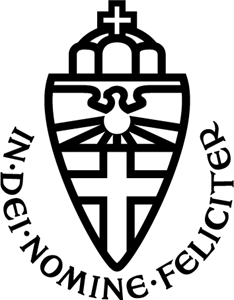
\includegraphics[height=1cm]{radboud}}

\begin{document}

\frame{\titlepage}

\begin{frame}
    \frametitle{Overview}
    \tableofcontents
\end{frame}

\section{Introduction}
\begin{frame}
    \frametitle{The path integral}
    \begin{equation}
        Z = \int \mathcal{D}[g_{\mu \nu}] e^{i S[g_{\mu \nu}]}
    \end{equation}
    \begin{equation}
        S[g_{\mu \nu}]
        =
        \frac{1}{16 \pi G}
        \int_\mathcal{M} \dd[d]{x} \sqrt{-g}
        (R(x) - 2 \Lambda)
    \end{equation}
    After simplifications: %TODO
    \begin{equation}
        Z = \sum_{T_\ell} \frac{1}{N_2(T_\ell)!} e^{-\lambda N_2(T_\ell)}
    \end{equation}
\end{frame}

\begin{frame}
    \frametitle{Volume fixing}
    Split $Z$ into fixed volume contributions
    \begin{equation}
        Z
        =
        \sum_{T_\ell} \frac{1}{N_2(T_\ell)!} e^{-\lambda N_2(T_\ell)}
        =
        \sum_{n = 0}^\infty \Omega(n) \frac{e^{-\lambda n}}{n!}
    \end{equation}
    Problem:
    \begin{itemize}
        \item $\lambda > \ln 2$: typical triangulation has a very small volume $\to$ cannot extract useful data
        \item $\lambda < \ln 2$: triangulation keeps growing $\to$ equilibrium cannot be reached
    \end{itemize}
    Our solution: fix the number of triangles $N_2$
\end{frame}



\end{document}